%%%%%%%%%%%%%%%%%%%%%%%%%%%%%%%%%%%%%%%%%%%%%%%%%%%%%%%%%%%%%%%%%%%%%%%%%%%%%%%

\chapter{PROPOSTA}\label{ch:prop}

Nesta seção apresentamos os objetivos do trabalho, bem exploramos a problemática dos dados disponíveis atualmente, e explicamos quais partes da estrutura do cubo de dados serão implementadas para resolver o problema.
\section{Objetivos}\label{ch:prop:obj}

O objeitvo principal deste trabalho é modelar os dados de telemetria de satélites em uma estrutura de cubo de dados, avaliando o uso da estrutura como uma abordagem para \textit{Big data}, assim permitindo a execução de análises e respostas a consultas que não seriam realísticas de outro modo. Como objetivos secundários, este trabalho visa:

\begin{enumerate}
\item Formalizar quais são as consultas relevantes para os operadores de satélite, e quais são as atividades de análise que podem ser expressas como consultas;
\item Criar uma representação dimensional do cubo de dados apropriada para as consultas identificadas, mapeando as medidas que são necessárias e quais os seus tipos;
\item Implementar a representação com as medidas em algoritmos da literatura e coletar os resultados da execução das consultas relevantes para os operadores;
\item Avaliar os resultados da implementação dos algoritmos e mostrar qual das abordagens é mais apropriada para o cenário da operação.
\end{enumerate}

Assim, nas próximas seções, é necessário qualificar o volume dos dados e porque uma abordagem tradicional não é adequada.

\section{Dados no INPE}\label{ch:prop:data}

Utilizando de uma estivativa sobre os dados já disponibilizados para este trabalho, a tabela~\ref{fig:datagenest} mostra a geração por ano de dados no CCS.
Essa estimativa foi feita utilizando dos dados não compressos a partir da disponibilidade dos mesmos.
Ela também assume que o Amazônia-1 vai gerar um volume de dados de telemetria similar ao gerado do CBERS.

\begin{figure}[!htb]
	\caption{Estimativa de geração anual de dados pelos satélites do INPE}\label{fig:datagenest}
	\vspace{4mm}
	\begin{center}
		\resizebox{15cm}{!}{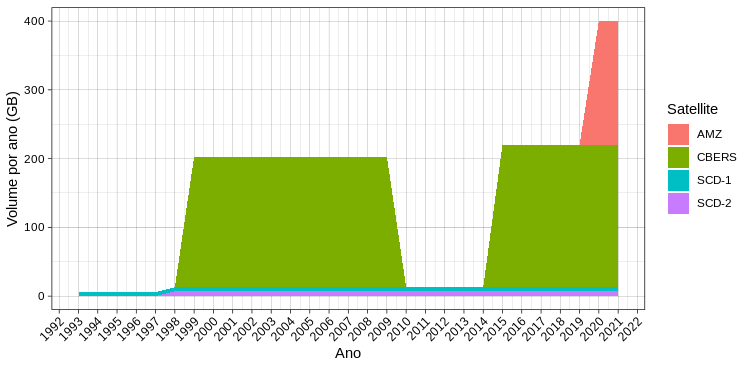
\includegraphics{Figuras/DataGenSatYear.png}}
	\end{center}
	\vspace{2mm}
	\legenda{}
	\FONTE{Produção dos autores.}
\end{figure}

Dessa estimativa, podemos obter o total de dados de telemetria disponíveis para a análise no CCS, apresentados na figura~\ref{fig:totaldatagen}.
É importante ressaltar que a grande maioria desses dados não está disponível para consulta pelo usuário, visto que somente os dados de alguns poucos anos da operação estão disponíveis para os operadores e engenheiros, necessitando de trabalho significativo para analisar dados do passado.

\begin{figure}[!htb]
	\caption{Estimativa do volume de dados históricos de telemetria}\label{fig:totaldatagen}
	\vspace{4mm}
	\begin{center}
		\resizebox{15cm}{!}{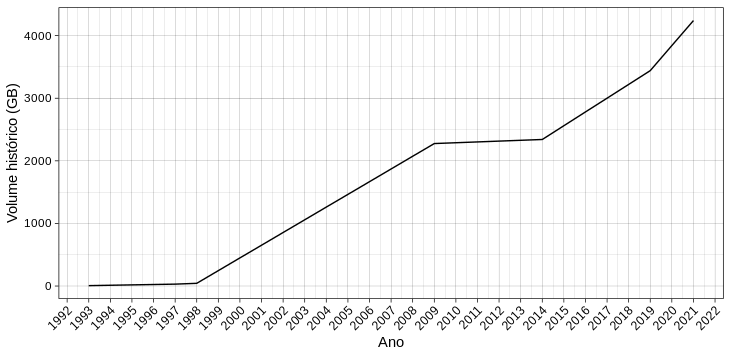
\includegraphics{Figuras/VolumeToYear.png}}
	\end{center}
	\vspace{2mm}
	\legenda{}
	\FONTE{Produção dos autores.}
\end{figure}

Essa oportunidade de pesquisa deve ser aproveitada para que os dados não virem ``\textit{dark data}'', que denota quaisquer tipo de dados que não são de fácil acesso para os usuários em potencial~\cite{heidornSheddingLightDark2008}.

Considerando que todos os dados já estivessem no banco de dados, propriamente formatados e prontos para a análise, ainda teríamos grandes problemas: com um banco de dados na ordem dos \textit{terabytes}, consultas multidimensionais ou que precisem de dados de vários anos poderiam demorar dias, ou mais, para serem executadas.
Para conseguir responder a consultas com desempenho satisfatório, propomos o uso de uma estrutura de cubo de dados neste trabalho.

\section{Cubo de Dados}\label{ch:prop:cubearch}

A figura~\ref{fig:cubearch} demonstra a divisão em 4 camadas de uma estrutura de Cubo de Dados.
Essas camadas demonstram tudo o que é necessário para a implementação de um Cubo de Dados, não sendo necessário que uma camada esteja fortemente atrelada a outra.

\begin{figure}[ht]
	\caption{Estrutura do Cubo de dados}\label{fig:cubearch}
	\vspace{6mm}
	\begin{center}
		\resizebox{10cm}{!}{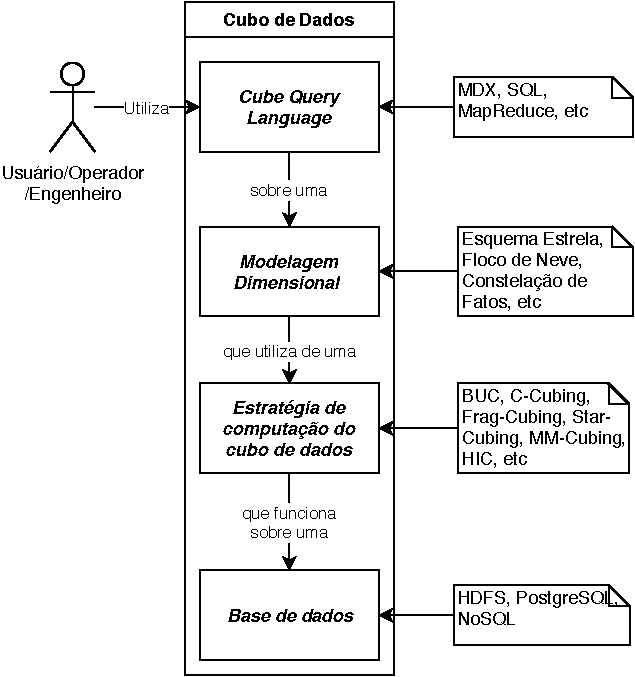
\includegraphics{Figuras/DataCubeArchitecture.pdf}}
	\end{center}
	\vspace{2mm}
	\legenda{}
	\FONTE{Produção dos autores.}
\end{figure}

Para esta proposta, vamos nos concentrar apenas na proposição de um algoritmo de computação do cubo de dados mais apropriado, utilizando das outras seções quando elas vão se tornando necessárias.
Os detalhes, algoritmos e conceitos listados na figura estão majoritariamente descritos na seção~\ref{ch:fun:cube}.

Uma informação interessante é que esta estrutura mostra o uso de pelo menos duas linguagens de computação sobre os dados: uma é a Cube Query Language que será utilizada pelo usuário para realizar as operações sobre o cubo (Drill-Down, Roll-up, etc), e outra é a linguagem que será utilizada pelo cubo para realizar essas operações, e elas podem ser independentes, por exemplo, pode-se utilizar SQL extendida com vocabulário de OLAP, porém o algoritmo de cubo de dados internamente pode consultar uma estrutura feita com MapReduce para o cálculo das medidas e das agregações.

Porém, utilizar duas linguagens muito diferentes nesse ponto pode não ser uma boa ideia, pois adicionaria um nível de diferença entre o usuário e os dados.
Caso seja necessário realizar uma consulta OLTP normal, sem o uso do cubo de dados, por exemplo, essa diferença ficaria mais óbvia, por exemplo traduzir uma consulta de SQL para MapReduce não seria muito fácil simplesmente por ter que entender de ambas as linguagens bem para conseguir fazer isso.
Deste modo, é interessante manter a mesma linguagem ao longo da estrutura, apenas alterando nas operações relevantes para o cubo de dados.

Com isso se torna necessário ressaltar o último nível, a Base de Dados: a escolha de banco de dados vai impactar como o algoritmo funciona, visto que existem diferentes sistemas de arquivos e como eles são atingidos, bem como o estilo do banco vai mudar como o algoritmo deve gerar o cubo, pois a base pode utilizar diferentes paradigmas de banco de dados~\cite{cuzzocreaDataWarehousingOLAP2013}.

\subsection{Algoritmos de construção do cubo}\label{ch:prop:cubearch:algo}

Uma das necessidades de usar algoritmos diferentes de cubo de dados está no número de dimensões que um certo cubo consegue realizar pesquisas: consultas com mais que 15 dimensões não são comummente(ou praticamente) executadas em alguns algoritmos, como o trabalho de~\cite{silva:2015:abordagensParaCubo} demonstra.

{\color{red}
Como estabelecido na seção~\ref{ch:prop:data}, os dados de telemetria de interesse possuem muito mais do que o limite de consultas em até 60 dimensões: com mais de 130 telemetrias para os satélites da família da SCD, e milhares para satélites maiores, a execução de consultas complexas seria normalmente inviável nos algortimos de construção do cubo.
}
Esse problema é geralmente resolvido pela modelagem dimensional, como em~\cite{AzevedoAmbr:2010:ArSaTe}, porém isso transforma os dados de um formato ``largo'' para um formato ``longo'', aumentando o número de tuplas.

Deste modo é necessário investigar as abordagens de construção de cubo que funcionem com muitas dimensões, e que permitam o cálculo das medidas necessárias para a operação.

{\color{red} Desenvolver mais sobre o algoritmos?}

